\documentclass{article}

% Package imports
\usepackage{titlesec}
\usepackage{geometry}
\usepackage{fancyhdr}
\usepackage{graphicx}
\usepackage{hyperref} % \url, https://www.overleaf.com/learn/latex/Hyperlinks

\geometry{a4paper, includeheadfoot, portrait, total={}, top=12.5mm, bottom=12.5mm, left=25.4mm, right=25.4mm}

\graphicspath{ {./images/} }

% Variables
\def\projectname{Computer Science NEA}

% Override subparagraph with a variant that has no indentation
% https://tex.stackexchange.com/a/392014
\makeatletter
\renewcommand\subparagraph{%
\@startsection{subparagraph}{5}{0pt}%
{3.25ex \@plus 1ex \@minus .2ex}{-1em}%
{\normalfont\normalsize\bfseries}}
\makeatother

\title{\projectname}
\author{James Cahill}
\date{Sepetember 2023}

% Configure fancyHDR page style
% https://tex.stackexchange.com/questions/266911/get-fancyhdr-and-geometry-to-work-nicely
\fancypagestyle{style}{
    \fancyhead{} % clear all header fields
    \fancyhead[HL]{\projectname}
    \fancyhead[HR]{James Cahill}
    \renewcommand{\headrulewidth}{0pt} % Remove header line
}
\pagestyle{style}


\begin{document}


\tableofcontents

\pagebreak

\section{Analysis}

% Background
\subsection{Problem Identification}

\subsubsection{Problem Description}

Popular inventory management solutions are relatively expensive, and may be out
of reach for individuals or small schools.
Inventory systems have numerous benefits for businesses and individuals alike; a business
may choose to track their supply levels where an individual may wish to catelogue their DVD collection. \\

\noindent My goal is to create a web-based application aimed at both businesses and individuals to manage
inventory, with additional modern features such as automatic item re-ordering when stocks are running low.\\

\noindent Traditional inventory management solutions are typically single-user at best, whereas I am to create
a multi-user, collaborative environment.


An inventory system should be able to:

time consuming to add data
not user friendly

- be easy to use (intuitive)
- catalogue of inventory, re-order for you
- be cross-platform, Fast
- scan using a phone (no external hardware needed)
- alert / re-order when stocks are running low.
- purchase links
- stretch: source data from amazon or equivalent instead of typing it manually
- search engine for catalogued and new Parts
    - provides with options for where to purchase certain goods
- button to re-order
    - smart device???????
- predict when stocks will run out.
- support for consumable and non-consumable goods.
- source data from external sources
- like monzo projection of when it will run out
- how much you are spending each month on goods
- nfc support to easily scan / etc items (migght be too hard on iOS)



\textbf{Barcode check in / out}

- monzo integration

- budgeting - figure projections  as well 

clearly define what the APP will feature.

Think about

- potenttial users
    - how does the app cater to their needs - different features etc




\subsubsection{Interview}

\subsubsection{Existing similar solutions}

% do 4-5 alternatives

\paragraph{\\InvenTree}
\url{https://inventree.org/}

\subparagraph{\\Overview\\}

InvenTree is an \textbf{open-source} inventory management system, providing \textit{low level stock control and part tracking}.
It uses a Python/Django database backend and provides both a \textbf{web-based interface} as well as a REST API for interacting with other services.
InvenTree also has a powerful plugin system for custom applications and other extensions. \\

\noindent Below is a screenshot of the InvenTree homepage.\\
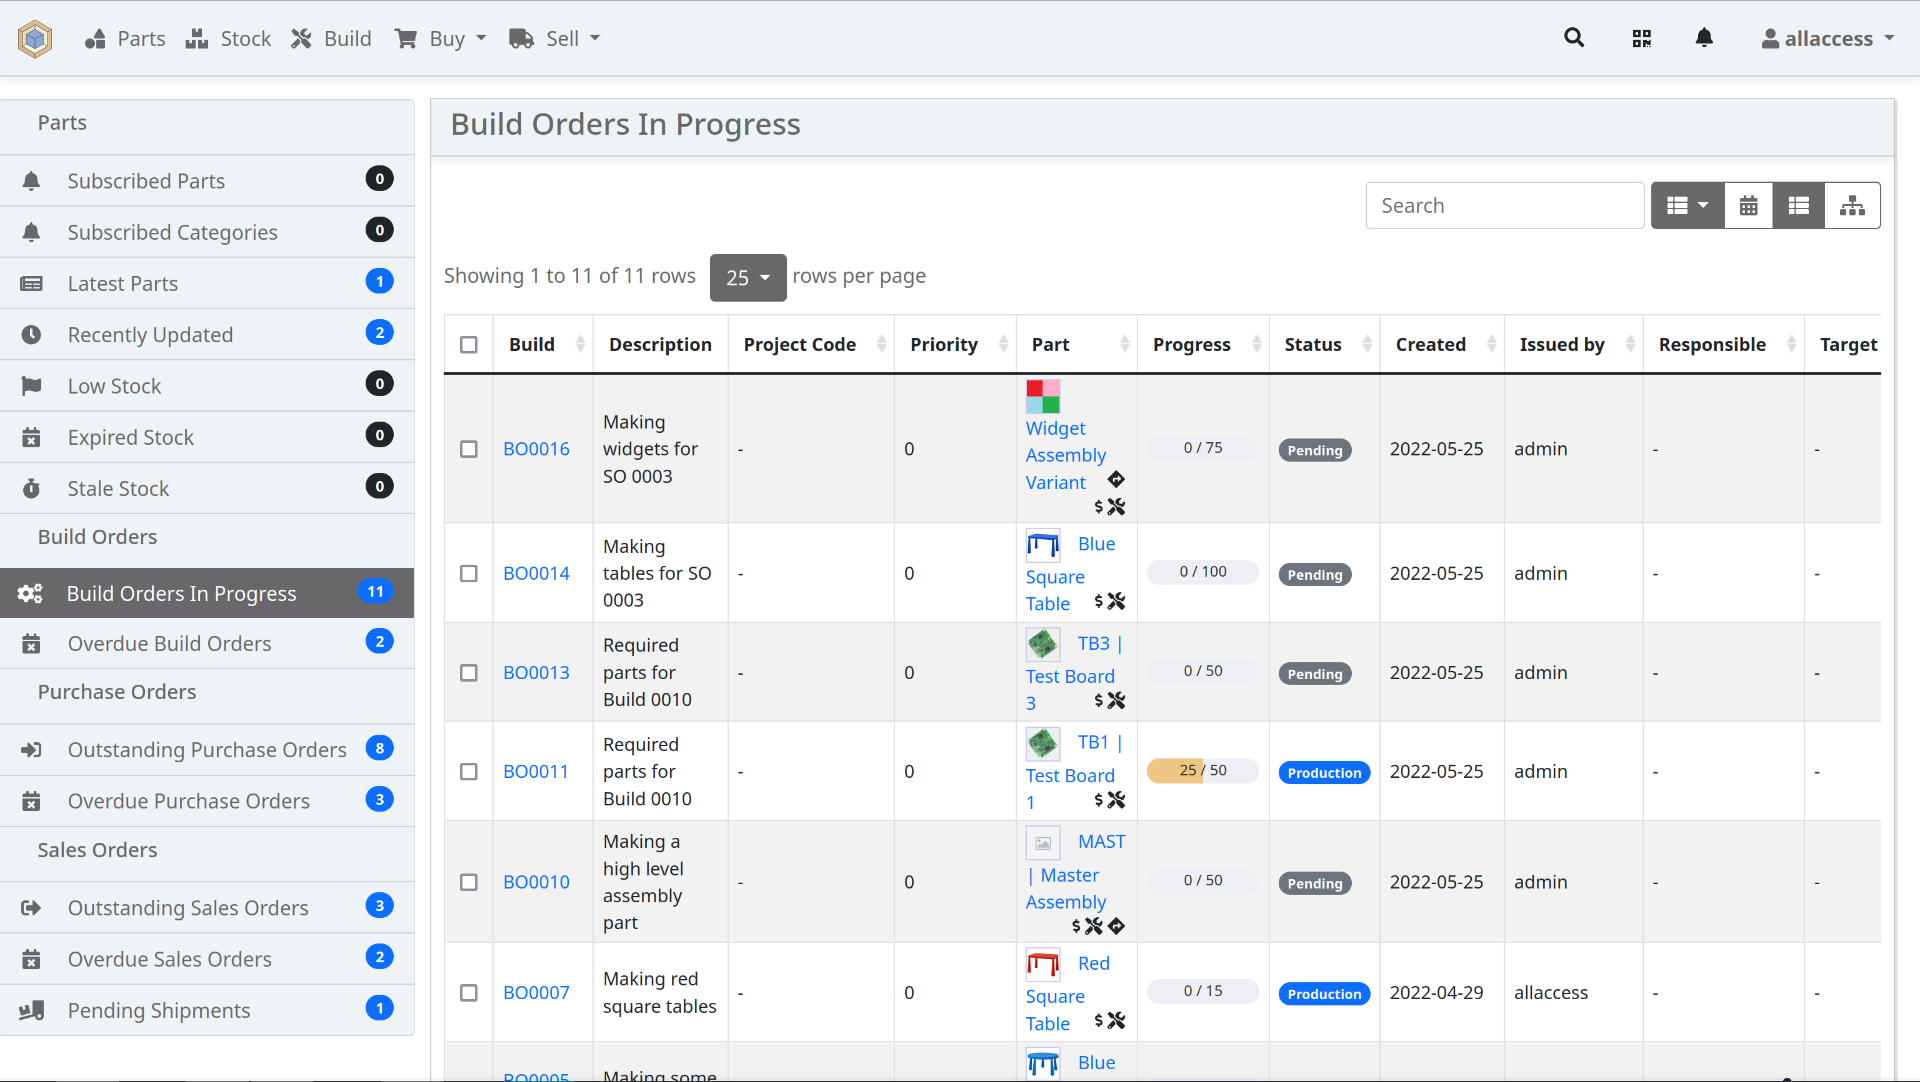
\includegraphics[width=15cm]{inventree_demo_homepage.png}

\subparagraph{Parts applicable to my solution\\}

- concept is similar (web-based), but I'm doing a different approach.\\
\noindent - not indented for stock control

\paragraph{\\PartKeepr}
\url{https://partkeepr.org/}\\

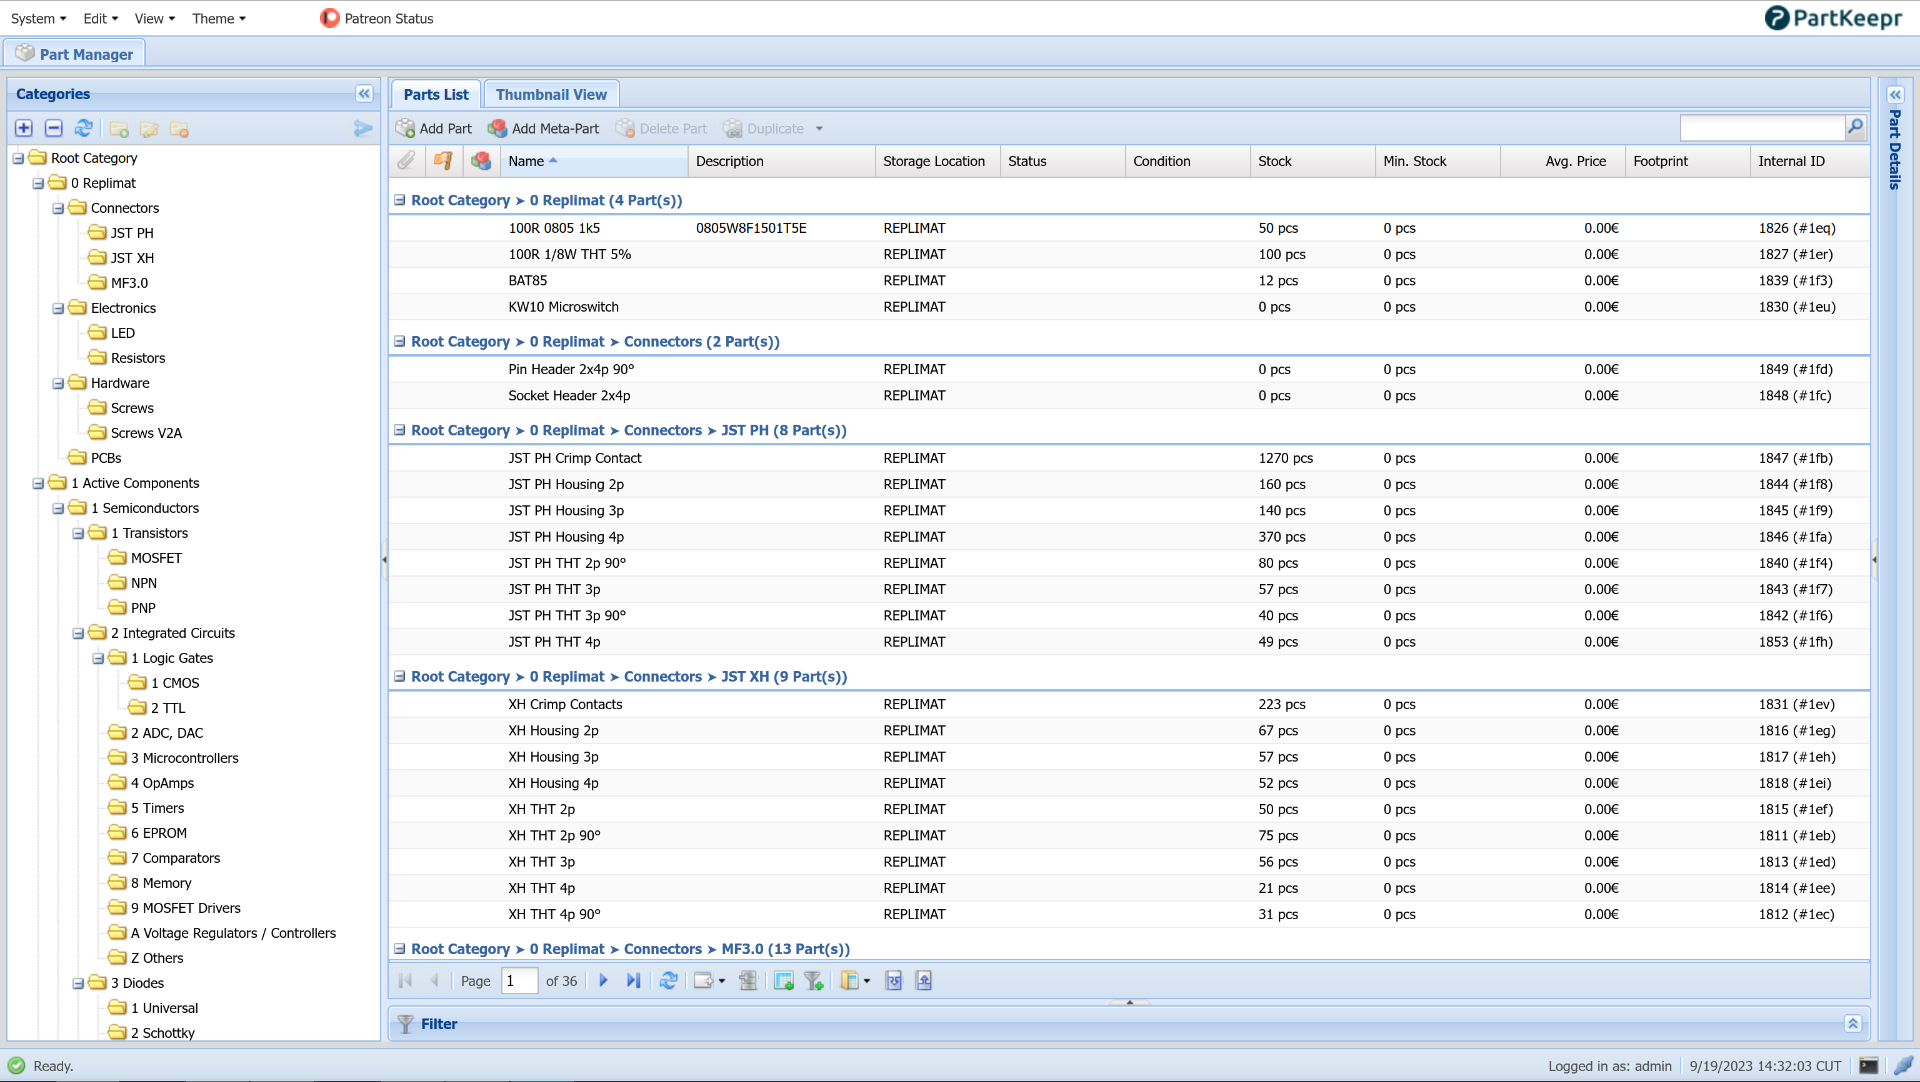
\includegraphics[width=15cm]{partkeepr_demo_homepage.png}

\subparagraph[indent=false]{\\Overview\\}

PartKeepr is an open-source inventory management system with a focus on electronic components.
It is designed around four main principles:

\begin{itemize}
    \item Fast Part Searching
    \item Ability to add complete part database
    \item Keeping track of stock
    \item Ease of use
\end{itemize}

\subparagraph{Parts applicable to my solution\\\\}

Like PartKeepr, I hope to implement a web-based interface.\\
However, I am using a different approach as my solution will not be tailored specifically to
electronic components.

\paragraph{\\Sortly}
\url{https://www.sortly.com/solutions/inventory-management-software/}\\

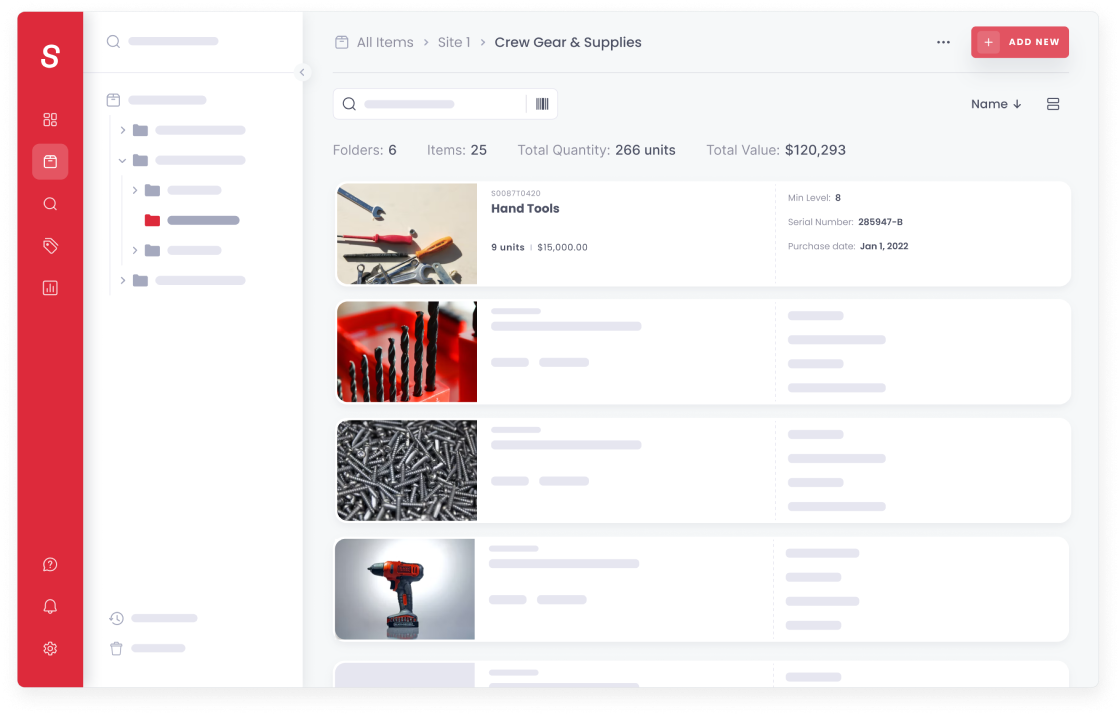
\includegraphics[width=15cm]{sortly_homepage_mockup_1.png}

\subparagraph{\\Overview\\}

Sortly is a proprietary cloud-based inventory management system with a focus on small businesses and inviduals.\\\\
It has two plans available, an always free plan with limited functionality and a paid plan will a more complete feature-set.

\subparagraph{Parts applicable to my solution\\\\}

I hope to implement the following features from Sortly:

\begin{itemize}
    \item Web based interface
    \subitem Allows for easy access.

    \item Ability to create QR codes to stick on items/containers
    \subitem Allows for easily unit selection in the interface.

    \item Real-time reporting insights
    \subitem 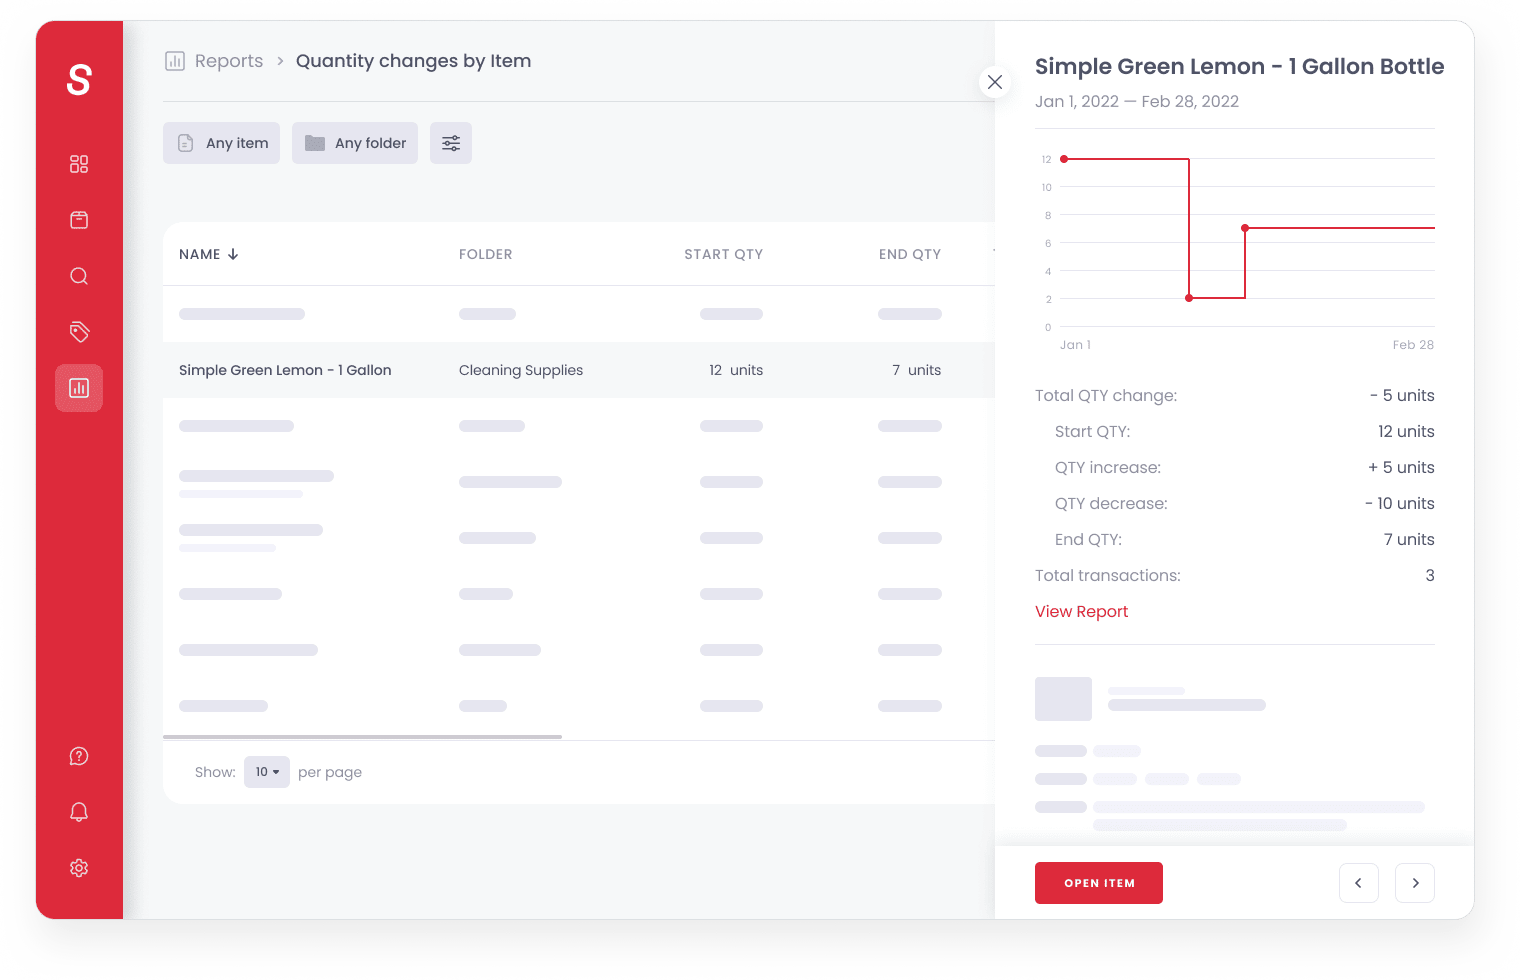
\includegraphics[width=10cm]{sortly_homepage_mockup_2.png}
    \subitem Allows for added insight into usage patterns for particular units.
\end{itemize}

\subsubsection{Features to be incorporated into solution}

\subsubsection{Feedback from stakeholders}

\subsection{Requirements}

\subsubsection{Stakeholder requirements}

\subsubsection{Software and hardware requirements}

\subsubsection{Success requirements}

\section{Design}

\subsection{User Interface Design}

\subsubsection{Usability Features}

\subsubsection{Feedback from stakeholder}

\subsection{Modular breakdown}

\subsection{Algorithms}

\subsection{Data Dictionary}

\subsection{Inputs and outputs}

\subsection{Validation}

\subsection{Testing}

\subsubsection{Methods}

\subsubsection{Test Plan}

\section{Implementation}

\subsection{First Iteration}

\section{Testing}

\section{Evaluation}

\end{document}